\documentclass[14pt]{extbook}
\usepackage{multicol, enumerate, enumitem, hyperref, color, soul, setspace, parskip, fancyhdr} %General Packages
\usepackage{amssymb, amsthm, amsmath, latexsym, units, mathtools} %Math Packages
\everymath{\displaystyle} %All math in Display Style
% Packages with additional options
\usepackage[headsep=0.5cm,headheight=12pt, left=1 in,right= 1 in,top= 1 in,bottom= 1 in]{geometry}
\usepackage[usenames,dvipsnames]{xcolor}
\usepackage{dashrule}  % Package to use the command below to create lines between items
\newcommand{\litem}[1]{\item#1\hspace*{-1cm}\rule{\textwidth}{0.4pt}}
\pagestyle{fancy}
\lhead{Module2}
\chead{}
\rhead{Version C}
\lfoot{3163-1865}
\cfoot{}
\rfoot{test}
\begin{document}

\begin{enumerate}
\litem{
Write the equation of the line in the graph below in Standard form $Ax+By=C$. Then, choose the intervals that contain $A, B, \text{ and } C$.
\begin{center}
    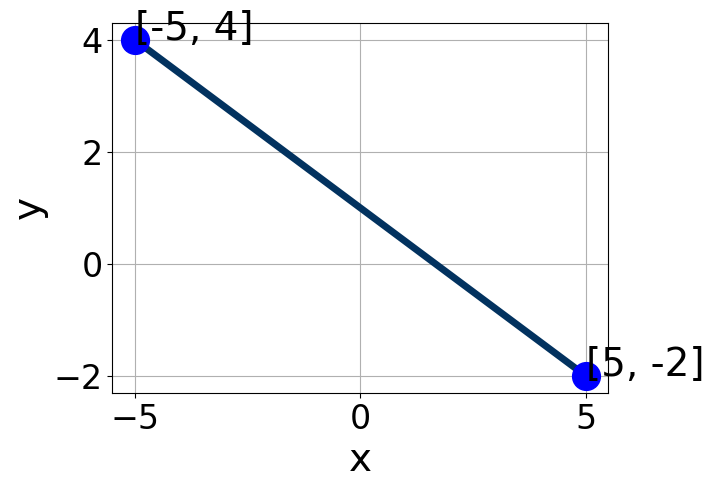
\includegraphics[width=0.5\textwidth]{../Figures/linearGraphToStandardC.png}
\end{center}
\begin{enumerate}[label=\Alph*.]
\item \( A \in [2.6, 4.4], \hspace{3mm} B \in [3.5, 8.3], \text{ and } \hspace{3mm} C \in [10, 16] \)
\item \( A \in [-4.4, -2.3], \hspace{3mm} B \in [-5.5, -2.5], \text{ and } \hspace{3mm} C \in [-16, -13] \)
\item \( A \in [-0.1, 2.9], \hspace{3mm} B \in [-2.8, -0.9], \text{ and } \hspace{3mm} C \in [-8, 0] \)
\item \( A \in [-0.1, 2.9], \hspace{3mm} B \in [0.2, 2.2], \text{ and } \hspace{3mm} C \in [2, 7] \)
\item \( A \in [2.6, 4.4], \hspace{3mm} B \in [-5.5, -2.5], \text{ and } \hspace{3mm} C \in [-16, -13] \)

\end{enumerate} }
\litem{
First, find the equation of the line containing the two points below. Then, write the equation as $ y=mx+b $ and choose the intervals that contain $m$ and $b$.\[ (3, -5) \text{ and } (-11, 8) \]\begin{enumerate}[label=\Alph*.]
\item \( m \in [-2.1, 0.9] \hspace*{3mm} b \in [-2.29, -1.64] \)
\item \( m \in [-2.1, 0.9] \hspace*{3mm} b \in [1.73, 2.37] \)
\item \( m \in [0.6, 3.8] \hspace*{3mm} b \in [17.97, 18.25] \)
\item \( m \in [-2.1, 0.9] \hspace*{3mm} b \in [-8.98, -5.83] \)
\item \( m \in [-2.1, 0.9] \hspace*{3mm} b \in [18.24, 20.96] \)

\end{enumerate} }
\litem{
Solve the equation below. Then, choose the interval that contains the solution.\[ -2(-4x + 15) = -18(-10x -12) \]\begin{enumerate}[label=\Alph*.]
\item \( x \in [-1.06, -0.85] \)
\item \( x \in [-1.6, -1.15] \)
\item \( x \in [-1.11, -1.02] \)
\item \( x \in [0.98, 1.3] \)
\item \( \text{There are no real solutions.} \)

\end{enumerate} }
\litem{
Find the equation of the line described below. Write the linear equation as $ y=mx+b $ and choose the intervals that contain $m$ and $b$.\[ \text{Parallel to } 9 x + 8 y = 14 \text{ and passing through the point } (-2, -3). \]\begin{enumerate}[label=\Alph*.]
\item \( m \in [-0.91, -0.2] \hspace*{3mm} b \in [-5.36, -5.07] \)
\item \( m \in [-1.25, -1.02] \hspace*{3mm} b \in [-5.36, -5.07] \)
\item \( m \in [0.75, 1.8] \hspace*{3mm} b \in [-0.86, -0.73] \)
\item \( m \in [-1.25, -1.02] \hspace*{3mm} b \in [5.13, 5.58] \)
\item \( m \in [-1.25, -1.02] \hspace*{3mm} b \in [-1.15, -0.99] \)

\end{enumerate} }
\litem{
Write the equation of the line in the graph below in Standard form $Ax+By=C$. Then, choose the intervals that contain $A, B, \text{ and } C$.
\begin{center}
    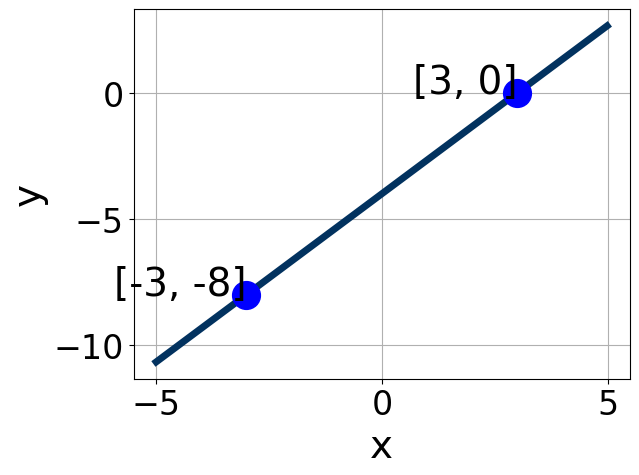
\includegraphics[width=0.5\textwidth]{../Figures/linearGraphToStandardCopyC.png}
\end{center}
\begin{enumerate}[label=\Alph*.]
\item \( A \in [2, 6], \hspace{3mm} B \in [2.02, 3.02], \text{ and } \hspace{3mm} C \in [2.82, 3.85] \)
\item \( A \in [2, 6], \hspace{3mm} B \in [-3.62, -1.76], \text{ and } \hspace{3mm} C \in [-3.04, -2.27] \)
\item \( A \in [-8, -4], \hspace{3mm} B \in [2.02, 3.02], \text{ and } \hspace{3mm} C \in [2.82, 3.85] \)
\item \( A \in [-3.67, 0.33], \hspace{3mm} B \in [-2.06, -0.84], \text{ and } \hspace{3mm} C \in [-2.46, 0.84] \)
\item \( A \in [-3.67, 0.33], \hspace{3mm} B \in [0.78, 2.33], \text{ and } \hspace{3mm} C \in [0.85, 1.3] \)

\end{enumerate} }
\litem{
Find the equation of the line described below. Write the linear equation as $ y=mx+b $ and choose the intervals that contain $m$ and $b$.\[ \text{Parallel to } 8 x - 3 y = 6 \text{ and passing through the point } (6, -9). \]\begin{enumerate}[label=\Alph*.]
\item \( m \in [0.6, 3.2] \hspace*{3mm} b \in [-17, -10] \)
\item \( m \in [0.6, 3.2] \hspace*{3mm} b \in [23, 26] \)
\item \( m \in [0.3, 1.7] \hspace*{3mm} b \in [-30, -23] \)
\item \( m \in [-4.9, -2.3] \hspace*{3mm} b \in [3, 9] \)
\item \( m \in [0.6, 3.2] \hspace*{3mm} b \in [-30, -23] \)

\end{enumerate} }
\litem{
First, find the equation of the line containing the two points below. Then, write the equation as $ y=mx+b $ and choose the intervals that contain $m$ and $b$.\[ (-8, 9) \text{ and } (2, -3) \]\begin{enumerate}[label=\Alph*.]
\item \( m \in [-2.9, -0.5] \hspace*{3mm} b \in [-5.01, -4.59] \)
\item \( m \in [-2.9, -0.5] \hspace*{3mm} b \in [16.67, 17.07] \)
\item \( m \in [-2.9, -0.5] \hspace*{3mm} b \in [-1.06, -0.5] \)
\item \( m \in [-2.9, -0.5] \hspace*{3mm} b \in [0.51, 0.76] \)
\item \( m \in [0, 1.7] \hspace*{3mm} b \in [-5.5, -5.09] \)

\end{enumerate} }
\litem{
Solve the linear equation below. Then, choose the interval that contains the solution.\[ \frac{-8x + 9}{4} - \frac{-6x + 3}{7} = \frac{-8x -5}{6} \]\begin{enumerate}[label=\Alph*.]
\item \( x \in [-57.75, -55.75] \)
\item \( x \in [-14.94, -9.94] \)
\item \( x \in [-19.44, -16.44] \)
\item \( x \in [-2.44, 4.56] \)
\item \( \text{There are no real solutions.} \)

\end{enumerate} }
\litem{
Solve the linear equation below. Then, choose the interval that contains the solution.\[ \frac{-7x + 8}{3} - \frac{-3x + 3}{2} = \frac{-9x + 4}{8} \]\begin{enumerate}[label=\Alph*.]
\item \( x \in [-13.07, -12.15] \)
\item \( x \in [-0.35, 0.8] \)
\item \( x \in [-3.53, -2.81] \)
\item \( x \in [-3.23, -1.57] \)
\item \( \text{There are no real solutions.} \)

\end{enumerate} }
\litem{
Solve the equation below. Then, choose the interval that contains the solution.\[ -16(-13x + 8) = -19(12x -14) \]\begin{enumerate}[label=\Alph*.]
\item \( x \in [0.51, 1.39] \)
\item \( x \in [6.33, 7.34] \)
\item \( x \in [-0.71, 0] \)
\item \( x \in [0.24, 0.65] \)
\item \( \text{There are no real solutions.} \)

\end{enumerate} }
\end{enumerate}

\end{document}